\chapter{Preliminary results}
Here the activities and results from the first year activities are registered. This section details the contacts established, projects and conferences 



\section{Contacts and meetings}
A set of stakeholders and potential data holders were contacted for collaboration. Institutions and actors from the Netherlands, Sweden, Portugal and Argentina were contacted. Conversations with some of these actors will continue during the following months to improve the needs of practitioners and what information could be used to populate the data model. In the table below the status of the contacts is highlighted. 
\begin{figure}[h!]
    \centering
    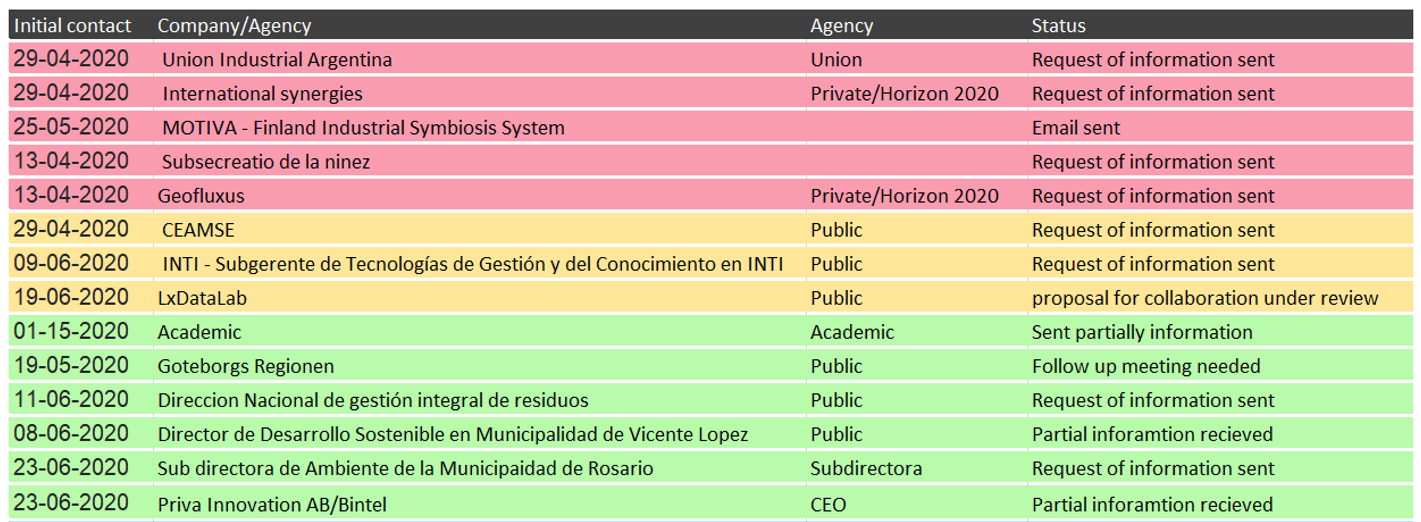
\includegraphics[width=0.95\textwidth]{sections/asset/contacts.PNG}
    \caption{Contacted stakeholders for collaboration}
    \label{fig:collaboration}
\end{figure}

The list of main potential partners are listed below:
\begin{enumerate}
    \item Dsposal (UK)
    \item Urban Metabolism group from WET at Chalmers (SWE)
    \item CEAMSE (ARG) 
\end{enumerate}


% \subsection{Household Waste}
% 13-04-2020: https://www.buenosaires.gob.ar/desarrollohumanoyhabitat/institucional-subsecretaria-de-ninez-y-adolescencia \par
% 29-04-2020: https://www.buenosaires.gob.ar/ciudadverde/separacion/porque-debemos-separar/programa-sello-giro\par
% 08-06-2020: Director de Desarrollo Sostenible en Municipalidad de Vicente Lopez \par

% \subsection{Industrial Associations contacted}
% 29-04-2020: https://www.uia.org.ar/medio-ambiente-y-desarrollo-sustentable/institucional/\par
% 29-04-2020: https://www.international-synergies.com/what-we-do/for-research/\par
% 29-04-2020: https://www.ceamse.gov.ar/generadores-privados/\par
% 05-05-2020: Informal data request to CEAMSEhttps://www.overleaf.com/project/5ea1c1fe57aac30001c2e0ec\par
% 25-05-2020: Marian Chertow\par
% 25-05-2020: MOTIVA - Finland Industrial Symbiosis System\par
% 08-06-2020: Director de Desarrollo Sostenible en Municipalidad de Vicente Lopez \par
% 09-06-2020: INTI - Subgerente de Tecnologías de Gestión y del Conocimiento en INTI \par
% 11-06-2020: Director de Desarrollo Sostenible en Municipalidad de Vicente Lopez \par
% 11-06-2020: Director de Desarrollo Sostenible en Municipalidad de Vicente Lopez \par
% 11-06-2020: CEAMSE \par
% 11-06-2020: Ex-director Nacional de gestión integral de residuos en el gobierno anterior: Luis Lehmann\par
% 19-06-2020: Subsecretaria de Ambiente de Rosario: Natalia Feldman\par

\section{Publications}

\subsubsection{A top-down method to support the identification of opportunities for Industrial Symbiosis partnerships}
Industrial Symbiosis (IS) can reduce industrial waste as well as the need for virgin material extraction by utilizing waste generated by one industry as raw material for another. Input-Output Matching is a commonly used method for identification of potential IS partnerships. In order to collect the data necessary to identify such opportunities, companies need to participate in activities such as workshops, surveys, or online questionnaires. However, these activities can be costly and time consuming. Additionally, companies may be unwilling to participate due to issues around data confidentiality. This article aims to show how these barriers can be overcome by a new method for identification of IS opportunities, which does not require companies to be surveyed. The developed matching approach makes use of statistical datasets and IS databases. The underlying principle is to use known IS partnerships and databases containing data on typical waste generation and resource use by industries to identify and link potential donors and receivers with similar characteristics, operating in other industry sectors. This allows expansion of a single IS case into multiple potential relationships. The method promotes Circular Economy development by finding ways to utilize more secondary resources through connecting previously unrelated industry sectors. The method has been tested in the Västra Götaland region in Sweden, where the goal was to identify potential partnerships between industries that generate sawdust as a waste product and companies that may be able to utilize this in their industrial processes. 159,630 of a total of 6,726,534 potential symbiotic links identified by the method were shortlisted, using prioritization criteria reflecting an increased likelihood of symbiosis.

\subsubsection{Mapping the spatial distribution of the effects of urban traffic congestion: methodological exploration using web based services}
Sustainable transport systems are a necessary requirement to achieve efficient economic performance, enhance urban quality of life and diminish environmental costs. Congestion, a negative externality of mobility, is responsible for urban pollution, inefficiency and has adverse effects over individuals facing this problem. For these reasons, transport and city planning agencies have developed interests in defining and measuring transportation congestion. Although, different definitions and metrics have been used, congestion measurements are found aggregated at a city level or for particular road segments. This study proposes a methodology that produces information from a web traffic service to map traffic congestion within an urban area. The method is simple and generalizable enough to be adopted in different urban areas. This paper presents the analysis of four European cities (Amsertdam, Glasgow, Goteborg and Lisbon) and show that the conclusions are consistent with the results obtained from internationally recognized organizations such as INRIX and TomTom.


\subsubsection{10\% Seminar \& report}




% \subsubsection{25\% Seminar \& report}


%\subsubsection{Annotated bibliography}



\section{Other research activities}
\subsubsection{Historical map of Gothenburg}
\href{https://chalmers.shinyapps.io/Goteborg_historical/?_ga=2.267750478.1104859035.1597823961-1745043960.1597823961}{Historical map of Gothenburg web site}


\subsubsection{Co-Design cards for Workshops in COVID-19 Times}

\href{https://chalmers.shinyapps.io/Goteborg_historical/?_ga=2.267750478.1104859035.1597823961-1745043960.1597823961}{Co-Design Cards}

\subsubsection{101 Lives - 48H Hackathon}
Hackathon aimed to propose strategies to reduce traffic accidents. I engaged in two teams that were awarded winners. The conversations with the insure company continued and they invited the team members to do a presentation to the company. 

\subsubsection{Economic Networks at Oxford}
In June 2019, the Economic Networks Summer School took place at oxford were a variety of advances in networks, tools and applications were introduced. 